\documentclass[conference]{IEEEtran}
\IEEEoverridecommandlockouts

\usepackage{cite}
\usepackage{amsmath,amssymb,amsfonts}
\usepackage{graphicx}
\usepackage{booktabs}
\usepackage{multirow}
\usepackage{xcolor}
\usepackage{url}
\usepackage[hidelinks]{hyperref}
\graphicspath{{figures/}}

\newcommand{\sensor}[1]{\texttt{s\_#1}}

\begin{document}

\title{Remaining Useful Life Prediction for Turbofan Engines:\\
Degradation Feature Engineering with Classical Machine Learning}

\author{
\IEEEauthorblockN{Kushal Tyagi}
\IEEEauthorblockA{Enrollment No.\ 2401010249}
\and
\IEEEauthorblockN{Nishant Sharma}
\IEEEauthorblockA{Enrollment No.\ 2401010302}
\and
\IEEEauthorblockN{Anant Lalwani}
\IEEEauthorblockA{Enrollment No.\ 2401020086}
\and
\IEEEauthorblockN{Dev Tyagi}
\IEEEauthorblockA{Enrollment No.\ 2401010148}
\and
\IEEEauthorblockN{Vansh Khod}
\IEEEauthorblockA{Enrollment No.\ 2401010493}
\and
\IEEEauthorblockA{\textit{Newton School of Technology, Rishihood University}\\
Advanced Machine Learning · Project 7, Phase 1}
}

\maketitle

\begin{abstract}
Predicting how many operating cycles an engine has left before it fails is the core task of predictive maintenance. We study remaining useful life (RUL) prediction on the FD001 subset of NASA's C-MAPSS turbofan degradation data set and ask how far carefully engineered degradation features can take classical machine learning models. We build a leakage-free pipeline: features are strictly causal, everything learned from data is fitted on training engines only, and all validation is done with five-fold cross-validation grouped by engine. The 88 features include rolling statistics, least-squares trend slopes at two horizons, each engine's deviation from its own early-life baseline, and a principal-component health index, with operating-regime normalisation that we validate on FD002. Controlled experiments show that a piecewise-linear target capped at 125 cycles cuts error by 44\% compared with a linear target, and that the engineered features roughly halve the error of tree ensembles compared with raw sensor readings. On the official test set, a tuned XGBoost model reaches an RMSE of 10.75 cycles (95\% CI 9.1--12.4), compared with 18.2 on raw sensors. Its error in the last 50 cycles before failure is only 5.7 cycles. An error analysis shows the remaining weaknesses: fast-degrading engines, the onset of degradation, and short histories. These depend on the timing of the full trajectory and motivate the sequence models of Phase~2.
\end{abstract}

\begin{IEEEkeywords}
predictive maintenance, remaining useful life, C-MAPSS, feature engineering, gradient boosting, random forest, elastic net, SHAP
\end{IEEEkeywords}

%=====================================================================
\section{Introduction}
%=====================================================================
Unplanned engine failures are expensive and dangerous, while replacing parts on a fixed schedule wastes components that still have useful life. \emph{Condition-based} or \emph{predictive} maintenance replaces fixed schedules with decisions based on the measured health of each asset, and its central quantity is the remaining useful life (RUL): the number of operating cycles left before failure~\cite{lei2018review}.

Data-driven prognostics learns RUL directly from sensor histories of past units instead of from a physical degradation model. The NASA C-MAPSS data set~\cite{saxena2008damage,saxena2008dataset} has become the standard benchmark for this task: simulated engines with unknown initial wear degrade until failure while 21 sensors are recorded every cycle.

Project~7 compares two ways of using these sensors: (i) \emph{engineered degradation features} with classical regression models, and (ii) sequence models that learn directly from raw sensor windows. This report covers Phase~1, the classical machine-learning side. Our contributions are:
\begin{itemize}
  \item a leakage-free feature pipeline covering cycle, rolling mean, rolling slope, operating-regime and sensor-health features, with a test that proves the features are causal;
  \item controlled experiments on the target definition, feature groups, models and hyperparameters, all using engine-level cross-validation;
  \item an evaluation on the official test set with bootstrap confidence intervals, an error breakdown by degradation stage, and a SHAP interpretation;
  \item an analysis of where fixed-window features fail, which sets the baseline and the hypotheses for Phase~2.
\end{itemize}

%=====================================================================
\section{Related Work}
%=====================================================================
\textbf{Benchmark and early methods.} Saxena~\emph{et al.}~\cite{saxena2008damage} describe how C-MAPSS simulates damage propagation through an exponential degradation of flow and efficiency in the engine modules, and released the data for the PHM'08 challenge together with an asymmetric scoring function that penalises late predictions. The winning approach of that challenge was a similarity-based method that matches a test trajectory against a library of health-index curves of training engines~\cite{wang2008similarity}. Ramasso and Saxena~\cite{ramasso2014benchmark} later reviewed more than 70 publications using C-MAPSS and pointed out how inconsistent preprocessing and evaluation make results hard to compare.

\textbf{Target definition.} Heimes~\cite{heimes2008rnn} observed that degradation is barely visible early in life and proposed a \emph{piecewise-linear} RUL target that is constant at a maximum value before decreasing linearly. Most later work adopts this with a cap between 120 and 130 cycles.

\textbf{Feature engineering and sensor selection.} Coble and Hines~\cite{coble2009prognostic} formalised what makes a good prognostic parameter (monotonicity, prognosability and trendability), which we use to rank sensors. Health indices that fuse several sensors into one degradation signal are a common intermediate step~\cite{wang2008similarity,lei2018review}.

\textbf{Machine-learning models.} Random forests~\cite{breiman2001rf} and gradient boosting~\cite{friedman2001gbm}, in particular XGBoost~\cite{chen2016xgboost}, are strong general-purpose regressors for tabular features. The elastic net~\cite{zou2005elasticnet} combines L1 and L2 penalties and handles groups of correlated predictors, a property that matters for highly collinear engine sensors.

\textbf{Deep learning.} Babu~\emph{et al.}~\cite{babu2016cnn} applied convolutional networks to sensor windows, Zheng~\emph{et al.}~\cite{zheng2017lstm} used LSTMs~\cite{hochreiter1997lstm}, and Li~\emph{et al.}~\cite{li2018dcnn} reached an RMSE of 12.61 on FD001 with a deeper 1-D CNN. These models learn temporal patterns directly, which motivates Phase~2. A recurring question, which this phase addresses, is how much of their advantage remains against a well-engineered feature baseline evaluated under the same protocol.

%=====================================================================
\section{Data Set and Exploratory Analysis}
%=====================================================================
\subsection{The FD001 subset}
FD001 contains one operating condition (sea level) and one fault mode (high-pressure compressor degradation). The training set has 100 engines observed until failure (20,631 rows); the test set has 100 engines cut off at a random point before failure (13,096 rows), with the true RUL at the last observed cycle provided separately. Each row holds an engine id, a cycle index, three operational settings and 21 sensor readings. Training lifetimes range from 128 to 362 cycles (mean 206.3, std 46.3), while test engines are observed for 31 to 303 cycles (mean 131.0) and have a true RUL of 7 to 145 cycles. FD001 is well above the 3,000-row requirement of the project.

\subsection{Data quality}
We checked for missing, infinite and duplicated values, duplicated (engine, cycle) pairs, engines not starting at cycle~1, and gaps in the cycle sequence. All checks passed for both sets, so no imputation or row removal was needed. Six sensors (\sensor{1}, \sensor{5}, \sensor{10}, \sensor{16}, \sensor{18}, \sensor{19}) and \texttt{setting\_3} are constant, and \sensor{6} takes only two values. The remaining two settings vary only as tiny noise around zero, confirming a single operating regime. We keep the other \textbf{14 sensors}.

\subsection{Degradation behaviour}
Fig.~\ref{fig:traj} aligns all training engines at their failure point. Most sensors stay roughly constant for a long time and drift monotonically only in the final 100--150 cycles: temperatures (\sensor{2}, \sensor{3}, \sensor{4}), static pressure \sensor{11} and bypass ratio \sensor{15} rise, while HPC outlet pressure \sensor{7}, fuel-flow ratio \sensor{12} and the coolant bleeds \sensor{20}, \sensor{21} fall. The core speeds \sensor{9} and \sensor{14} behave differently across engines. Cycle-to-cycle noise is large: for \sensor{11} the noise standard deviation is about a tenth of the total change over life, so the trend cannot be seen from consecutive readings.

\begin{figure*}[t]
  \centering
  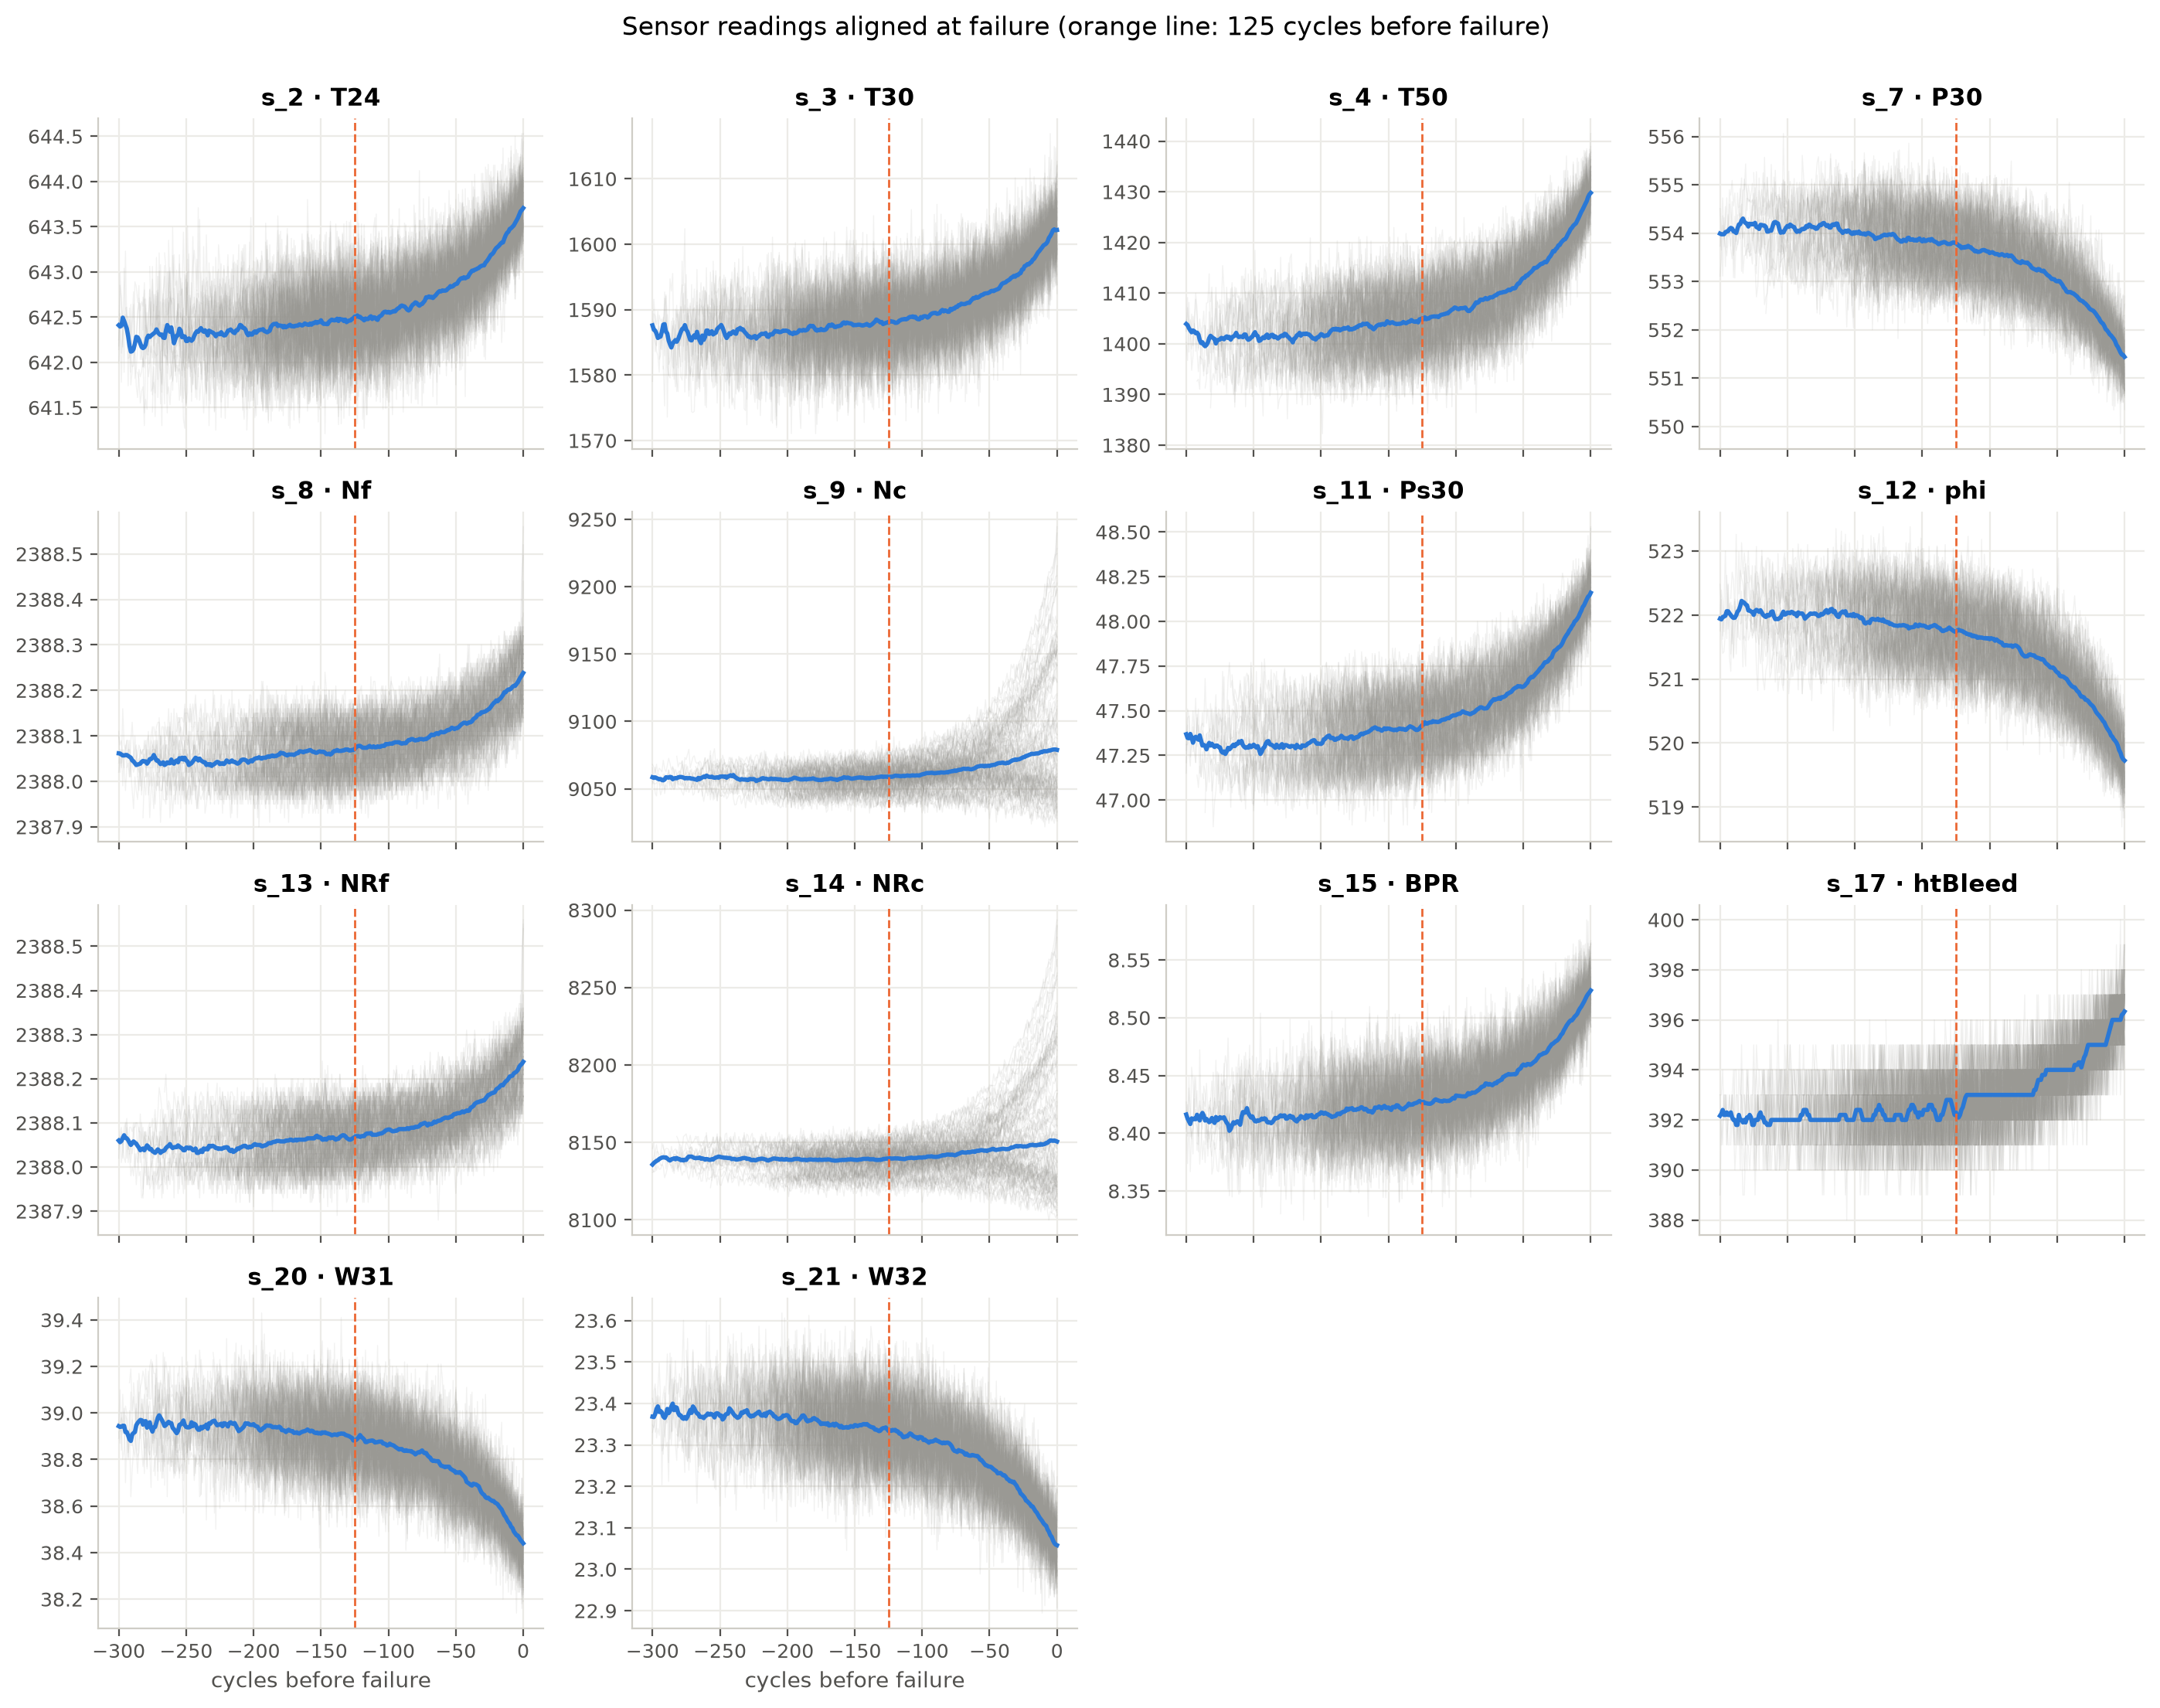
\includegraphics[width=0.92\textwidth]{02_sensor_trajectories.png}
  \caption{The 14 retained sensors for all training engines, aligned at failure (grey: individual engines; blue: median). Most sensors are flat early in life and trend over the last 100--150 cycles; the dashed line marks 125 cycles before failure.}
  \label{fig:traj}
\end{figure*}

\subsection{Sensor ranking}
Following~\cite{coble2009prognostic}, we computed monotonicity, trendability (mean absolute Spearman correlation with the cycle index) and prognosability on 20-cycle smoothed signals. \sensor{11}, \sensor{4} and \sensor{12} rank highest (average scores 0.73, 0.72 and 0.70), the core speeds \sensor{9} and \sensor{14} lowest among the kept sensors (0.49) because engines end at very different values, and the dropped \sensor{6} is worst on monotonicity and trendability. The sensors are strongly collinear: $|r|$ is often above 0.7, and $r=0.96$ between \sensor{9} and \sensor{14}.

\subsection{Implications for the target}
To locate the onset of visible degradation, we averaged the sign-aligned z-scores of the 14 sensors into one indicator. Its median across engines is flat until about 200 cycles before failure and reaches 10\% of its total rise at about 140 cycles before failure, accelerating thereafter (Fig.~\ref{fig:target}). Before this point the spread between engines is much larger than the change in the median, so the sensors carry little information about how much life is left. This supports a capped target, which we test formally in Section~\ref{sec:cap}.

\begin{figure}[t]
  \centering
  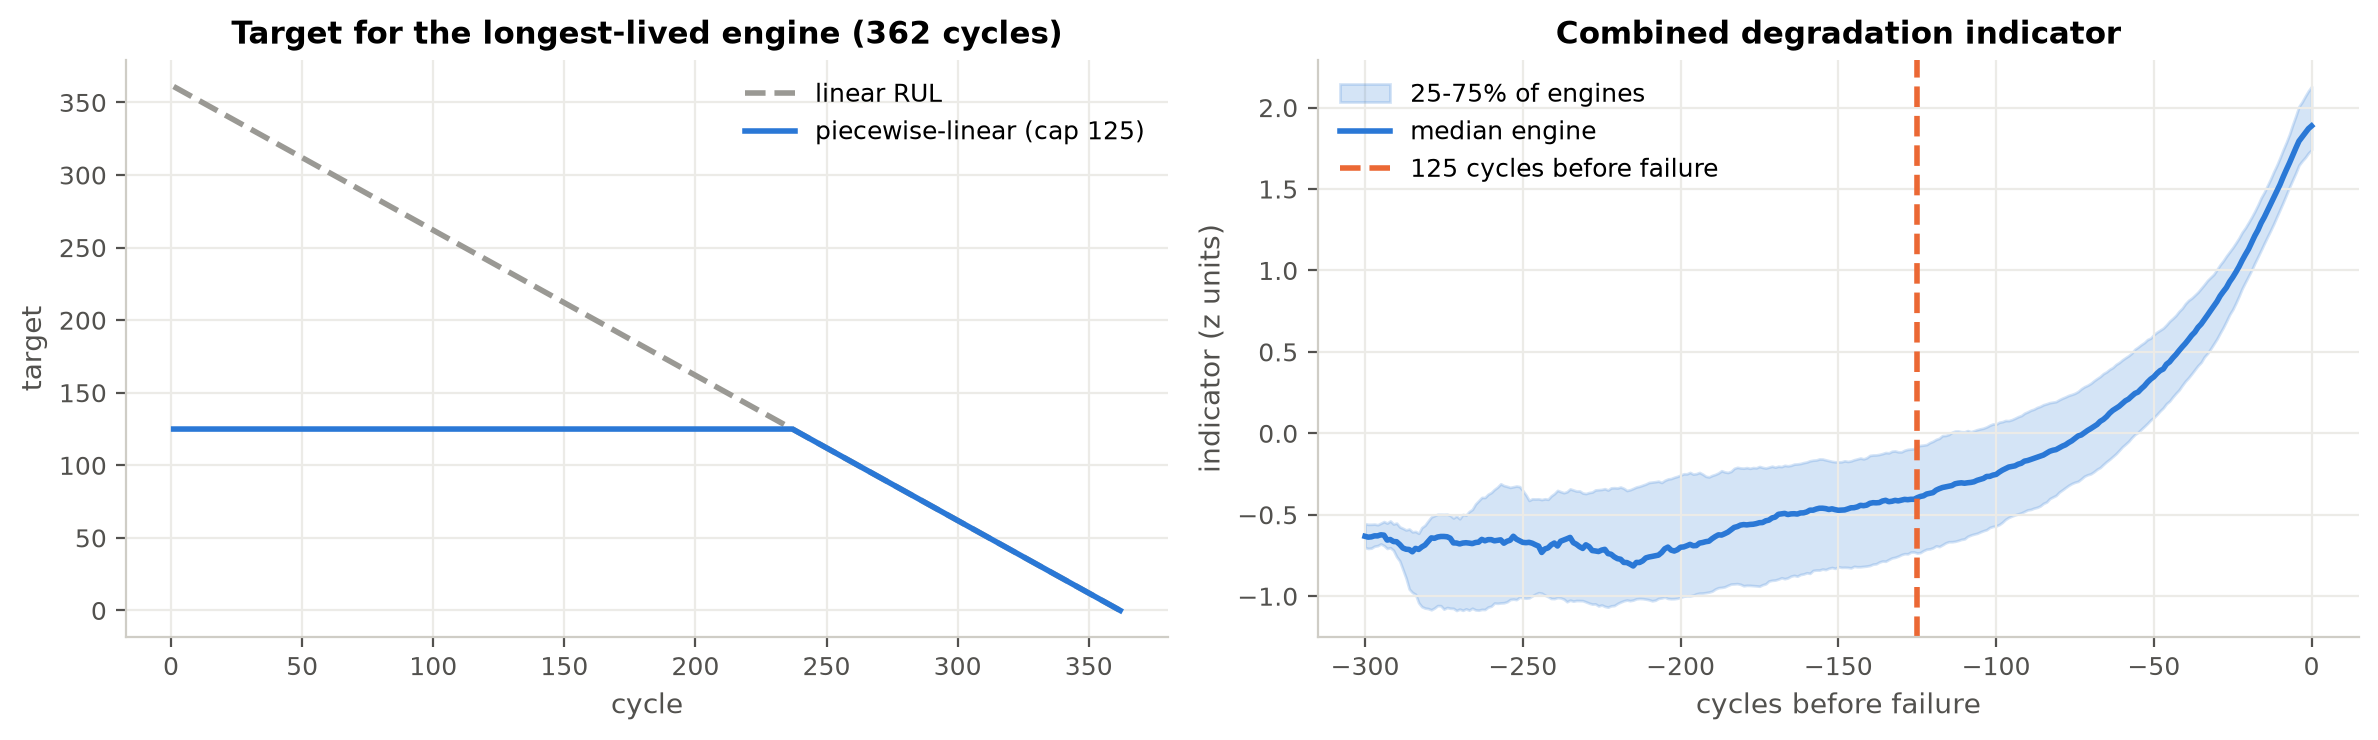
\includegraphics[width=\columnwidth]{02_target_choice.png}
  \caption{Left: linear vs.\ piecewise-linear target. Right: combined degradation indicator aligned at failure (median and interquartile band).}
  \label{fig:target}
\end{figure}

%=====================================================================
\section{Methodology}
%=====================================================================
\subsection{Problem formulation}
For training engine $i$ with last cycle $T_i$, the RUL at cycle $t$ is $\text{RUL}_{i,t}=T_i-t$. For a test engine, the given RUL at its last observed cycle $T^{\text{obs}}_i$ labels every earlier cycle as $\text{RUL}_{i,t}=\text{RUL}^{\text{last}}_i+(T^{\text{obs}}_i-t)$, which allows a per-stage evaluation. Models are trained on the piecewise-linear target
\begin{equation}
  y_{i,t}=\min\left(\text{RUL}_{i,t},\,R_{\max}\right),\qquad R_{\max}=125.
\end{equation}

\subsection{Feature engineering}
Every feature at cycle $t$ uses only cycles $1,\dots,t$ of the same engine, and every fitted transformation is fitted on training engines only. Inside cross-validation it is refitted on the training engines of each fold.

\textbf{Operating-regime normalisation.} The three settings are standardised and clustered with $k$-means; each sensor is then z-scored with the statistics of its own regime $r$:
\begin{equation}
  z_{i,t}=\frac{x_{i,t}-\mu_{r(i,t)}}{\sigma_{r(i,t)}}.
\end{equation}
On FD002 the silhouette score peaks clearly at $k=6$ (0.997), and normalisation removes the regime jumps that hide the degradation trend (Fig.~\ref{fig:regime}). FD001 has one regime, so the step reduces to a global z-score.

\begin{figure}[t]
  \centering
  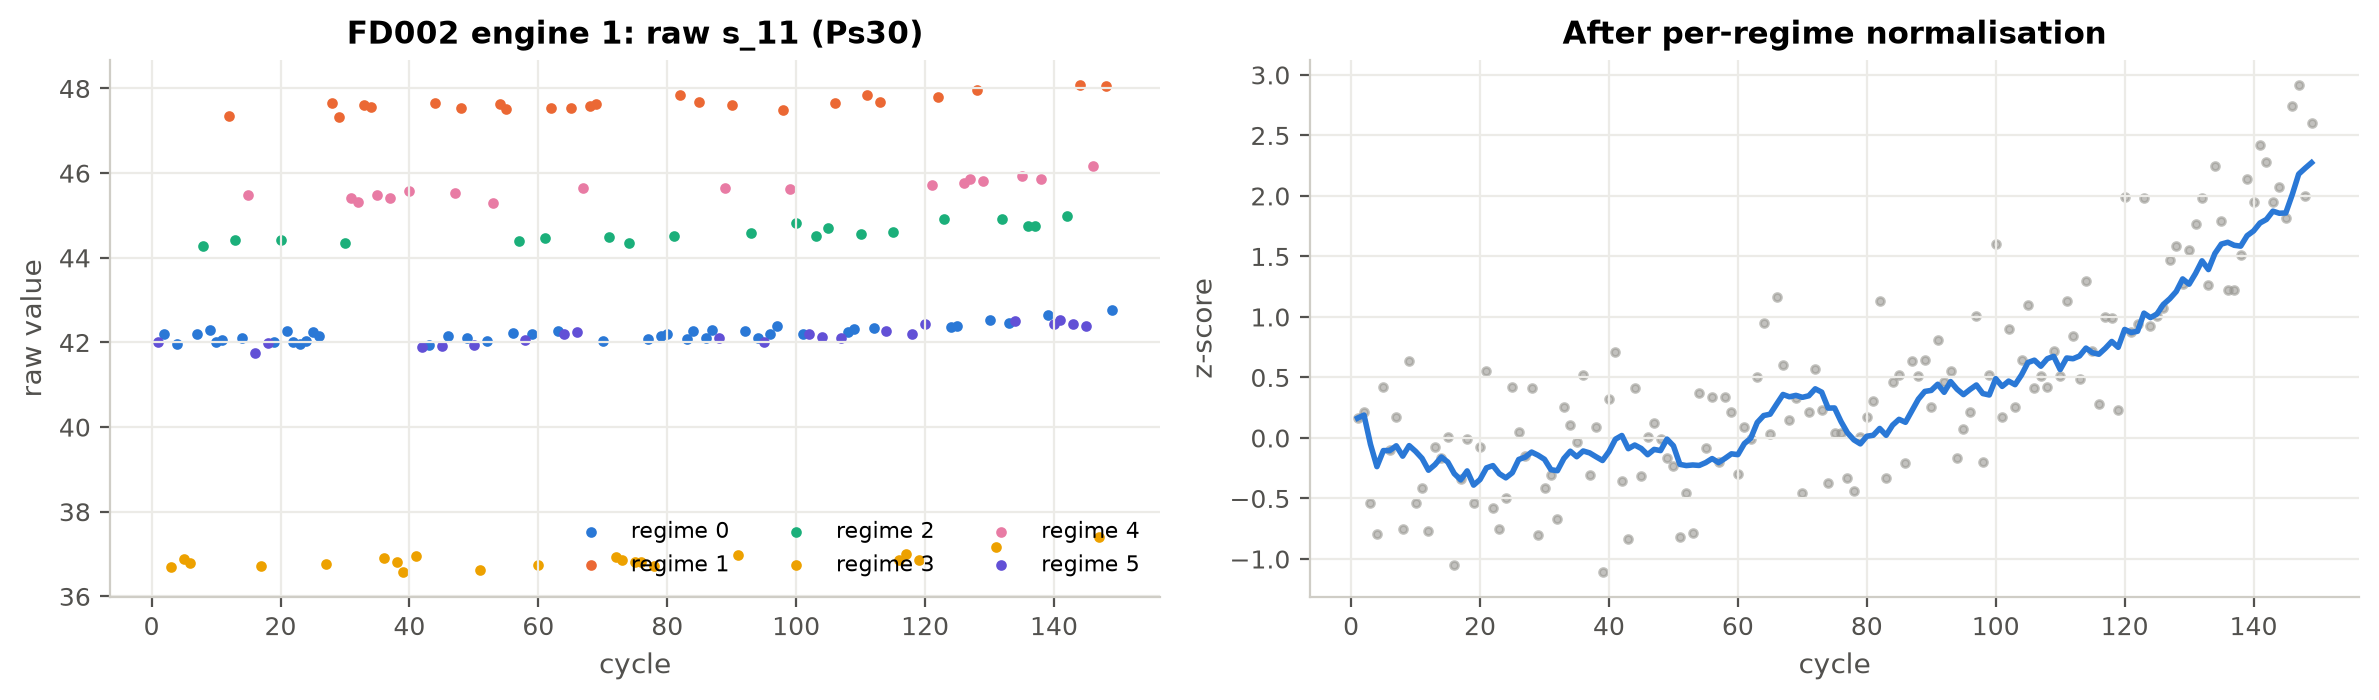
\includegraphics[width=\columnwidth]{03_regime_normalisation.png}
  \caption{FD002 engine 1: raw \sensor{11} jumps between six operating regimes (left); after per-regime normalisation the degradation trend becomes visible (right).}
  \label{fig:regime}
\end{figure}

\textbf{Feature groups.} With a short window $w=10$ and a long window $W=30$, we compute for each sensor: the normalised reading; its rolling mean and standard deviation over $w$; its rolling least-squares slope over $w$ and $W$,
\begin{equation}
  \hat\beta_t=\frac{\sum_{k=t-w+1}^{t}(k-\bar k)(z_k-\bar z)}{\sum_{k=t-w+1}^{t}(k-\bar k)^2};
\end{equation}
and the deviation of the rolling mean from the mean of the engine's first 10 cycles. We also add the current cycle $t$ and a health index: the first principal component of the 14 normalised sensors (64.3\% of the variance), sign-aligned to fall with age, together with its rolling mean and $W$-slope. The result is \textbf{88 features} with no missing values. Rolling standard deviations and slopes are set to zero until half a window of history exists, instead of being imputed. A truncation test, which recomputes features after deleting all future cycles, gives identical values (maximum difference $0$), confirming causality.

\subsection{Models}
\textbf{Elastic Net}~\cite{zou2005elasticnet} minimises
\begin{equation}
  \tfrac{1}{2n}\|y-X\beta\|_2^2+\alpha\left(\rho\|\beta\|_1+\tfrac{1-\rho}{2}\|\beta\|_2^2\right)
\end{equation}
on standardised features. The L1 term selects features and the L2 term stabilises correlated groups. \textbf{Random Forest}~\cite{breiman2001rf} averages deep regression trees grown on bootstrap samples with random feature subsets, which reduces variance. \textbf{XGBoost}~\cite{chen2016xgboost} adds shallow trees sequentially, each fitting the gradient of the loss, and minimises a regularised objective $\sum_j \ell(y_j,\hat y_j)+\sum_k\left(\gamma T_k+\tfrac{\lambda}{2}\|w_k\|^2\right)$ over the trees' leaf counts $T_k$ and leaf weights $w_k$. A mean predictor serves as the baseline.

\subsection{Evaluation protocol}
All model selection uses five-fold cross-validation over \emph{engine ids} (20 engines per fold). Splitting by row would place near-identical consecutive cycles of one engine on both sides and inflate the scores. The official test set is used once, at the end. With $d_j=\hat y_j-y_j$ we report RMSE (primary), MAE and the PHM'08 score~\cite{saxena2008damage}
\begin{equation}
  S=\sum_j\begin{cases}e^{-d_j/13}-1, & d_j<0\\ e^{d_j/10}-1, & d_j\ge 0,\end{cases}
\end{equation}
which penalises late predictions (over-estimated RUL) more heavily. Errors are further broken down into \emph{early} ($\text{RUL}>125$), \emph{mid} ($50<\text{RUL}\le125$) and \emph{late} ($\text{RUL}\le 50$) degradation stages. Hyperparameters are tuned by random search~\cite{bergstra2012random} on the cross-validation folds.

%=====================================================================
\section{Experiments and Results}
%=====================================================================
\subsection{Target design}\label{sec:cap}
We trained XGBoost on all features with a linear target and with caps from 100 to 175, and scored every variant against the \emph{true} RUL on validation cycles with $\text{RUL}\le150$, the region where maintenance decisions depend on the prediction (Table~\ref{tab:cap}). The linear target is clearly worst (RMSE 23.4). Caps of 125 and 140 are practically tied (13.2 and 13.3), and lower or higher caps degrade. We use $R_{\max}=125$, consistent with the onset analysis and with most published work.

\begin{table}[t]
\centering
\small
\setlength{\tabcolsep}{4pt}
\caption{Effect of the RUL cap (XGBoost, 5-fold CV, scored against true RUL)}
\label{tab:cap}
\resizebox{\columnwidth}{!}{\begin{tabular}{lccc}
\toprule
Cap & RMSE (RUL$\le$150) & MAE (RUL$\le$150) & RMSE (all) \\
\midrule
none (linear) & 23.42 & 15.00 & 36.46 \\
100 & 18.77 & 12.76 & 56.87 \\
115 & 14.44 & 10.16 & 49.52 \\
\textbf{125} & \textbf{13.17} & 9.37 & 45.43 \\
140 & 13.28 & \textbf{9.30} & 40.64 \\
155 & 14.66 & 10.12 & 37.18 \\
175 & 16.91 & 11.57 & 34.85 \\
\bottomrule
\end{tabular}}
\end{table}

\subsection{Raw sensors versus engineered features}
Table~\ref{tab:cv} compares every model on the 14 raw (normalised) sensors and on the 88 engineered features, with default hyperparameters. Engineered features reduce the cross-validation RMSE by 27\% for Elastic Net, 43\% for Random Forest and 49\% for XGBoost. On raw sensors, Random Forest and XGBoost perform almost identically, so the input representation, not the model, is the bottleneck. Elastic Net stays behind because a linear function cannot express the flat-then-declining target.

\begin{table}[t]
\centering
\small
\setlength{\tabcolsep}{4pt}
\caption{5-fold CV results (capped target, default hyperparameters)}
\label{tab:cv}
\resizebox{\columnwidth}{!}{\begin{tabular}{llcc}
\toprule
Model & Features & RMSE (mean $\pm$ std) & MAE \\
\midrule
Mean baseline & -- & 41.73 $\pm$ 0.20 & 37.01 \\
\midrule
\multirow{2}{*}{Elastic Net} & raw (14) & 21.28 $\pm$ 0.54 & 17.34 \\
 & engineered (88) & 15.62 $\pm$ 1.52 & 12.69 \\
\multirow{2}{*}{Random Forest} & raw (14) & 18.43 $\pm$ 0.61 & 13.56 \\
 & engineered (88) & 10.48 $\pm$ 1.13 & 7.03 \\
\multirow{2}{*}{XGBoost} & raw (14) & 18.57 $\pm$ 0.53 & 13.49 \\
 & engineered (88) & \textbf{9.48 $\pm$ 0.62} & \textbf{6.30} \\
\bottomrule
\end{tabular}}
\end{table}

\subsection{Feature-group ablation}
Fig.~\ref{fig:ablation} shows a forward ablation (adding one group at a time) and a leave-one-group-out ablation. For XGBoost, adding the cycle count lowers RMSE from 18.6 to 16.9, rolling statistics add little, slopes give the largest jump (to 12.0), baseline deviations another large gain (to 9.7), and the health index a final small one (to 9.5). Removing the cycle (+2.1) or the baseline deviations (+1.9) hurts most, while removing slopes changes nothing (0.0) because their information overlaps with the baseline deviations and the health-index slope. The most valuable information is therefore how far and how fast each engine has moved away from its \emph{own} early-life state, together with its age.

\begin{figure*}[t]
  \centering
  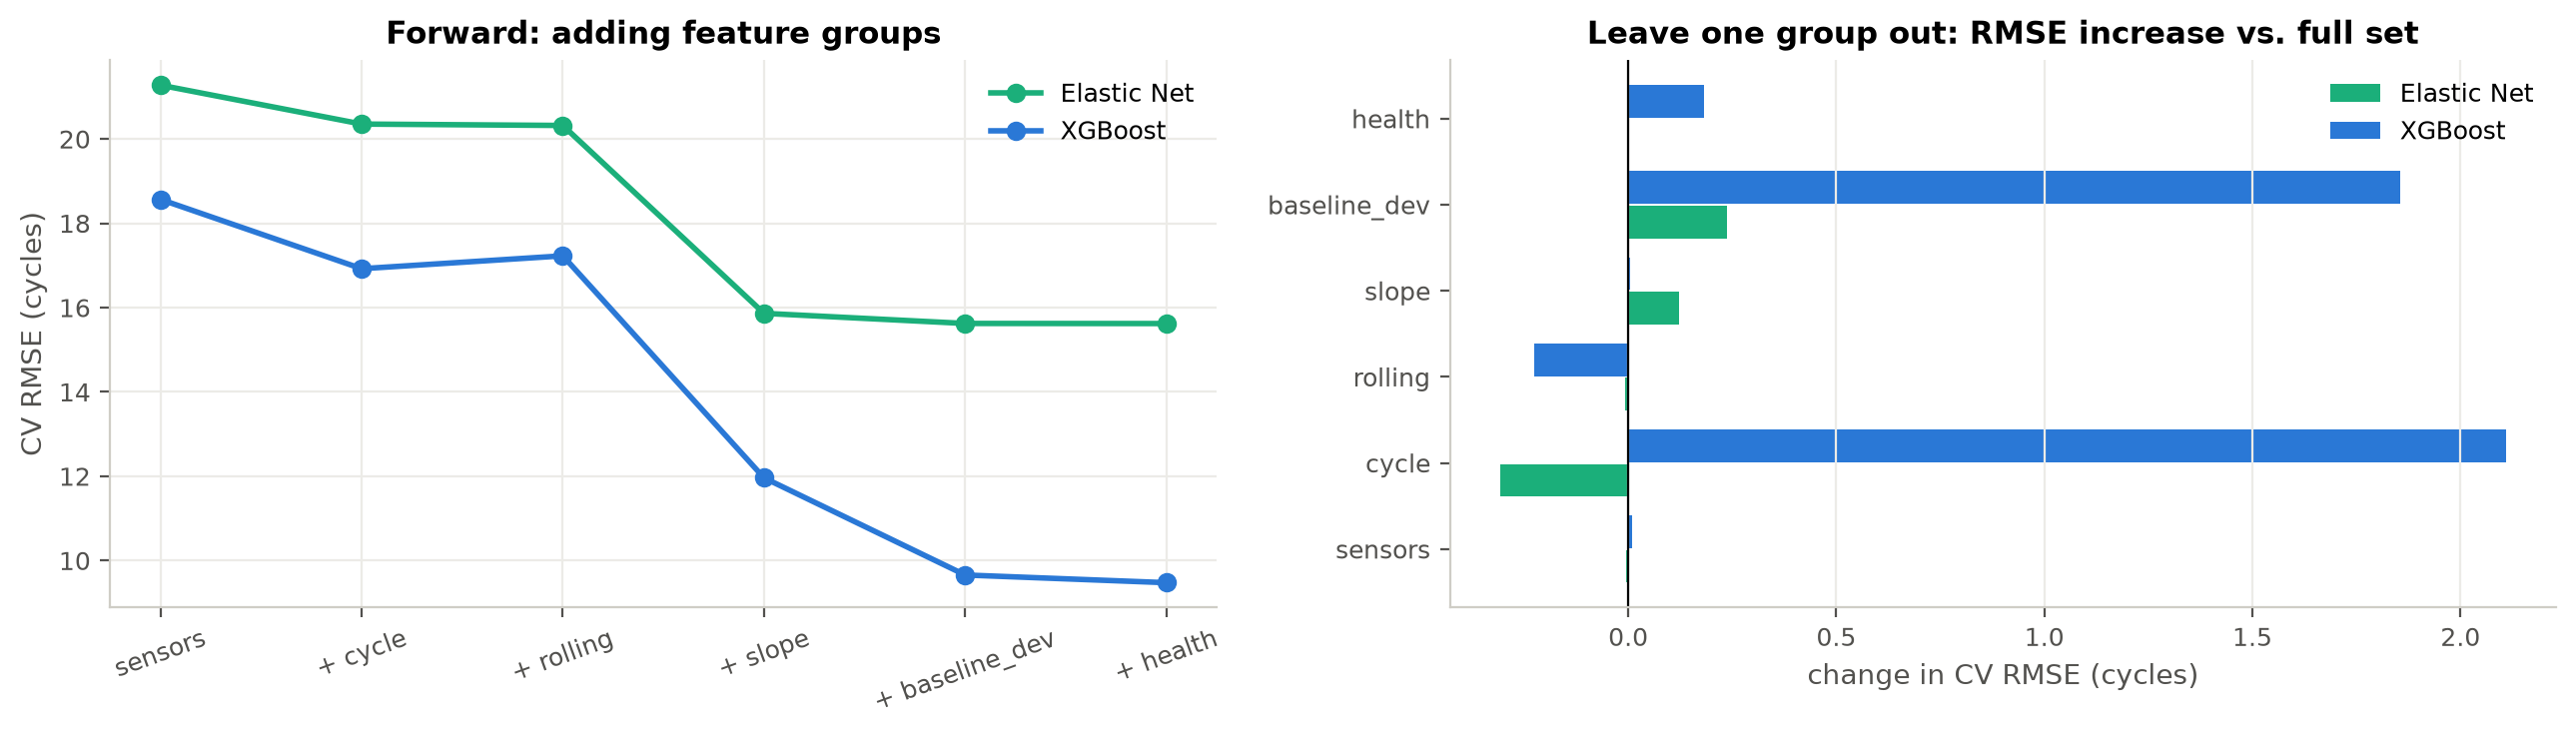
\includegraphics[width=0.85\textwidth]{04_feature_ablation.png}
  \caption{Feature-group ablation (5-fold CV RMSE). Left: groups added cumulatively. Right: RMSE change when one group is removed from the full set.}
  \label{fig:ablation}
\end{figure*}

\subsection{Hyperparameter tuning}
Random search improved XGBoost from 9.48 to $9.26\pm0.50$ (760 trees of depth 3, learning rate 0.09, minimum child weight 10, subsample 0.67, column sample 0.81) and Elastic Net from 15.62 to 15.41 ($\alpha=0.60$, $\rho=0.09$). It left Random Forest unchanged at about 10.5. XGBoost beats Random Forest on all five folds (by 1.25 cycles on average). Tuning contributes about 0.2 cycles, compared with about 9 cycles from feature engineering.

\subsection{Official test set}
The models are retrained on all 100 training engines and evaluated on the last cycle of each test engine against the true RUL (Table~\ref{tab:test}). The tuned XGBoost model reaches \textbf{RMSE 10.75} (95\% bootstrap CI 9.1--12.4), MAE 8.09 and $S=161$. The raw-sensor version scores 18.19 (CI 14.9--21.2), so the improvement is well outside sampling noise. The test RMSE agrees with the cross-validation estimate (9.69 against the capped truth versus 9.26 in CV), showing that the protocol gave a realistic estimate. For context, published FD001 results include an MLP (37.56), SVR (20.96), CNN (18.45)~\cite{babu2016cnn}, LSTM (16.14)~\cite{zheng2017lstm} and a deep CNN (12.61)~\cite{li2018dcnn}. Evaluation details differ between papers, so this comparison is indicative only, but it shows that the engineered baseline is strong. Fig.~\ref{fig:test} shows the predictions.

\begin{table}[t]
\centering
\small
\setlength{\tabcolsep}{4pt}
\caption{Official FD001 test set (last cycle, true RUL)}
\label{tab:test}
\resizebox{\columnwidth}{!}{\begin{tabular}{llccc}
\toprule
Model & Variant & RMSE [95\% CI] & MAE & Score \\
\midrule
Mean & -- & 43.07 [38.7, 47.5] & 35.90 & 33629 \\
\midrule
\multirow{2}{*}{Elastic Net} & raw & 21.90 [19.0, 24.7] & 17.62 & 1286 \\
 & eng.+tuned & 16.78 [14.7, 18.7] & 13.69 & 429 \\
\multirow{2}{*}{Rand.\ Forest} & raw & 18.07 [14.9, 20.9] & 13.19 & 829 \\
 & eng.+tuned & 11.91 [9.9, 13.9] & 8.79 & 197 \\
\multirow{2}{*}{XGBoost} & raw & 18.19 [14.9, 21.2] & 12.93 & 963 \\
 & eng.+tuned & \textbf{10.75 [9.1, 12.4]} & \textbf{8.09} & \textbf{161} \\
\bottomrule
\end{tabular}}
\end{table}

\begin{figure*}[t]
  \centering
  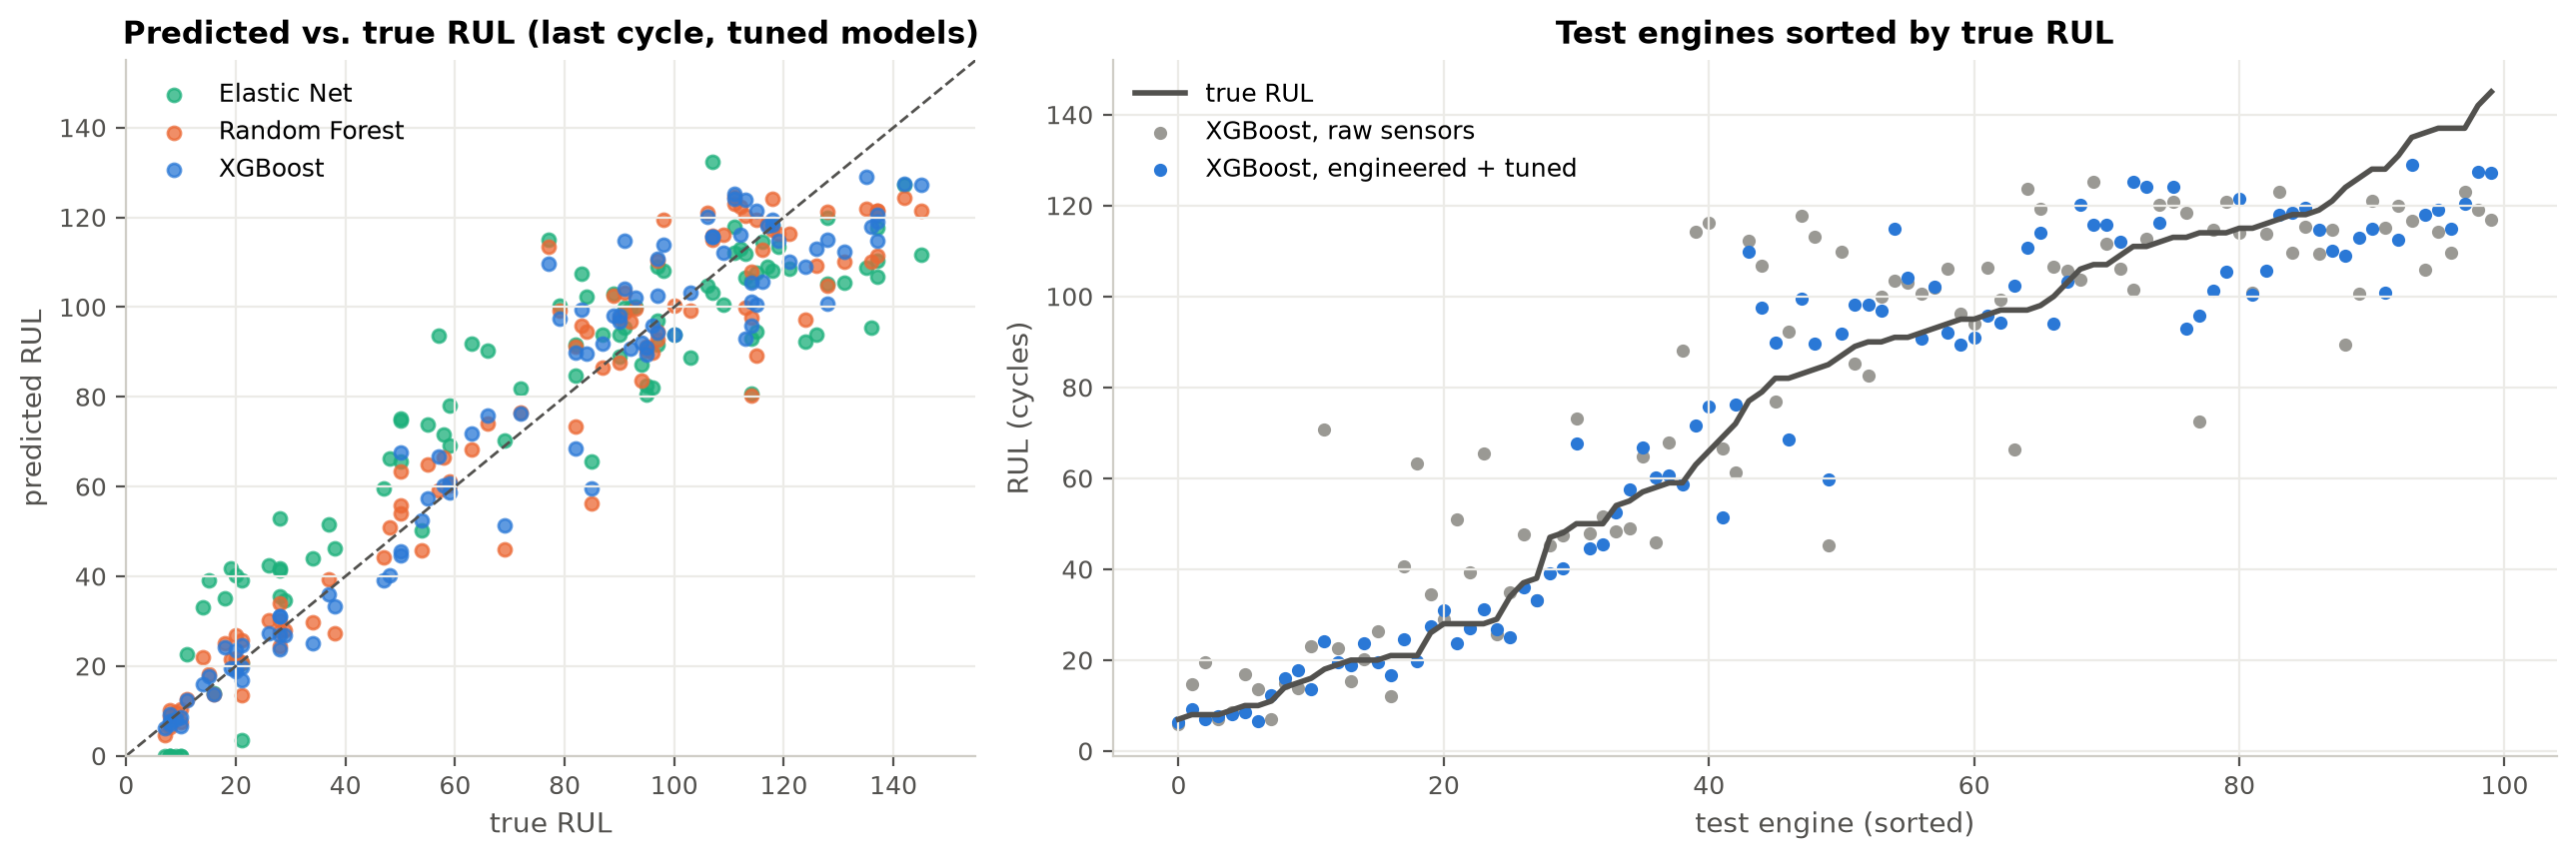
\includegraphics[width=0.9\textwidth]{05_test_predictions.png}
  \caption{Test-set predictions at the last observed cycle. Left: predicted vs.\ true RUL for the tuned models. Right: test engines sorted by true RUL; XGBoost with raw sensors (grey) vs.\ engineered features (blue).}
  \label{fig:test}
\end{figure*}

\subsection{Error by degradation stage}
Using all 13,096 test cycles (Table~\ref{tab:stage}, Fig.~\ref{fig:stage}), the engineered XGBoost model is most accurate where it matters most. In the late stage its RMSE is 5.7 with a bias of only $+2$ cycles, whereas the raw-sensor model has an RMSE of 28.8 and a late bias of $+17$ cycles, systematically over-estimating the life of failing engines. Elastic Net shows a similar late bias ($+16$). Mid-stage errors are higher (12.4) because degradation is only beginning there. Early-stage errors against the true RUL are large for every model, but by design: the models are trained to output the cap for healthy engines. Against the capped target, the engineered XGBoost model's early-stage RMSE is only 6.4 (raw: 12.3).

\begin{table}[t]
\centering
\small
\setlength{\tabcolsep}{4pt}
\caption{Test RMSE (bias) by stage, all test cycles, true RUL}
\label{tab:stage}
\resizebox{\columnwidth}{!}{\begin{tabular}{lccc}
\toprule
Model & Early & Mid & Late \\
\midrule
XGBoost, raw & 73.95 & 20.87 (+7.2) & 28.78 (+17.1) \\
Elastic Net, eng. & 72.57 & 15.88 (+3.6) & 20.34 (+15.9) \\
Random Forest, eng. & 69.39 & 13.50 (+2.3) & 7.46 (+3.3) \\
XGBoost, eng. & 68.38 & \textbf{12.44 (+2.7)} & \textbf{5.70 (+2.0)} \\
\midrule
$n$ (cycles) & 7952 & 4258 & 886 \\
\bottomrule
\end{tabular}}
\end{table}

\begin{figure}[t]
  \centering
  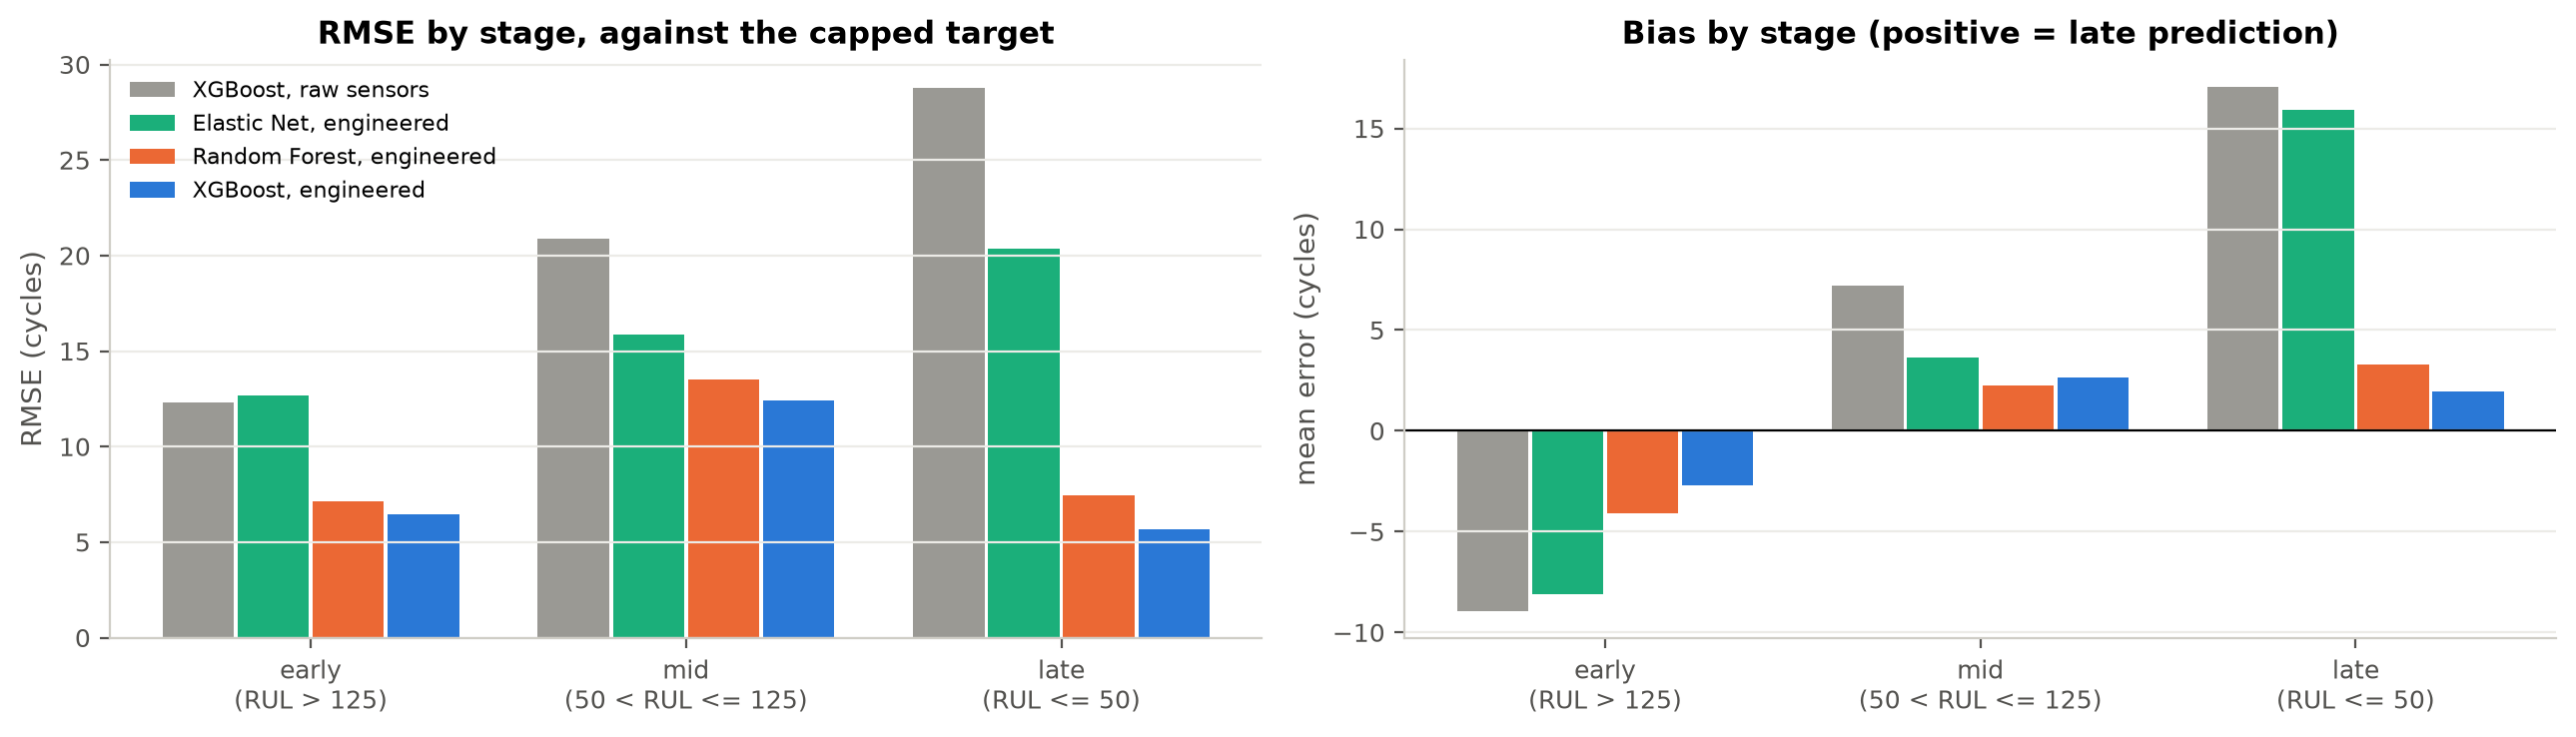
\includegraphics[width=\columnwidth]{05_error_by_stage.png}
  \caption{Test RMSE against the capped target (left) and bias (right) by degradation stage; positive bias means late (dangerous) predictions.}
  \label{fig:stage}
\end{figure}

\subsection{Interpretability}
TreeSHAP~\cite{lundberg2017shap} on the final XGBoost model (Fig.~\ref{fig:shap}) attributes most of the predictions to the baseline-deviation group, followed by the health-index features, rolling means and cycle. Raw readings contribute almost nothing once these are available. The single most important feature is the 30-cycle slope of the health index: a fast decline lowers the predicted RUL by up to about 25 cycles. Next come the baseline deviations of \sensor{11} and \sensor{4}, the two highest-ranked sensors in Section~III-D. A high cycle count \emph{raises} the prediction. Given the same amount of measured degradation, an engine that took longer to get there degrades slowly, so the model uses age to estimate the degradation \emph{rate}.

\begin{figure}[t]
  \centering
  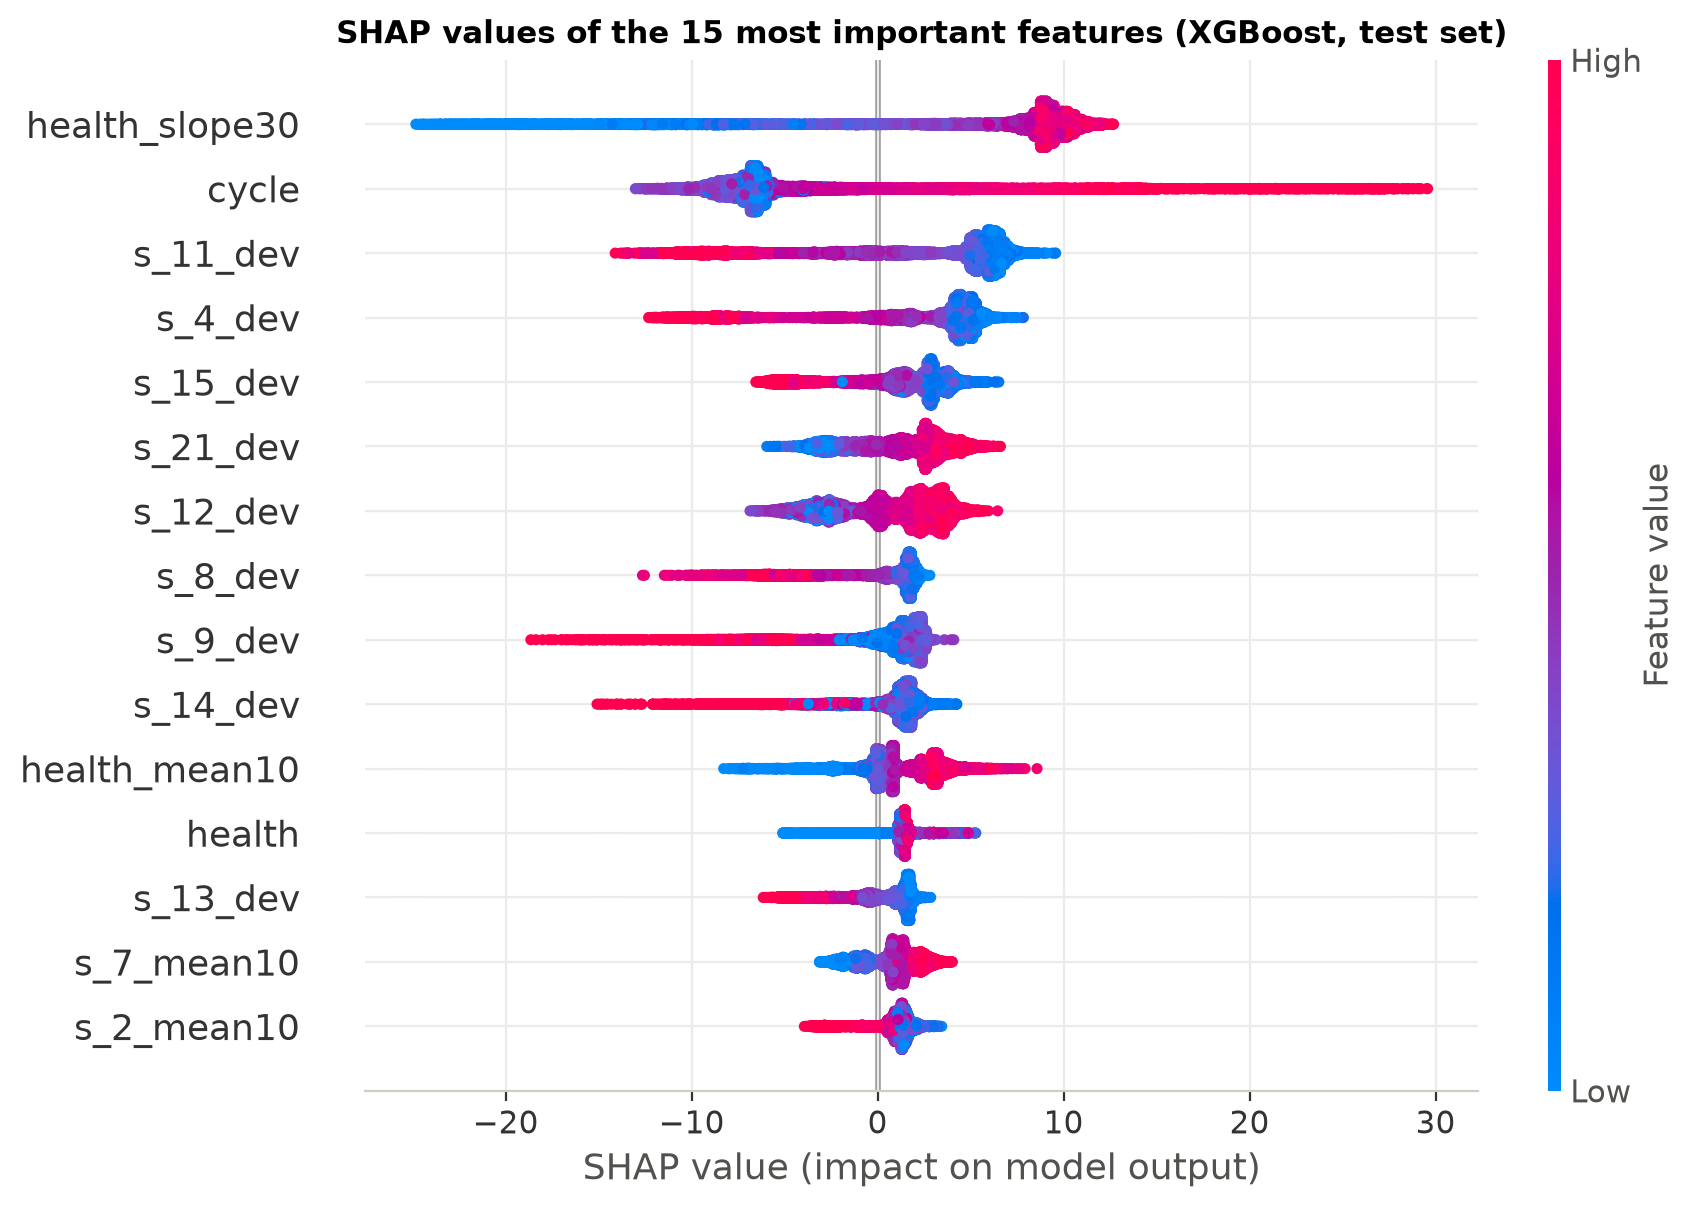
\includegraphics[width=\columnwidth]{05_shap_summary.png}
  \caption{SHAP values of the 15 most important features (XGBoost, test set). Colour shows the feature value; position shows its effect on the predicted RUL.}
  \label{fig:shap}
\end{figure}

%=====================================================================
\section{Discussion: Where Fixed Features Fall Short}
%=====================================================================
Using the out-of-fold predictions on training engines, we identified three systematic weaknesses (Fig.~\ref{fig:gap}). First, \textbf{fast-degrading engines}: per-engine error falls as lifetime grows (Spearman $\rho=-0.32$), and engines failing before 160 cycles are predicted late by about 10 cycles on average, against roughly zero bias for the others. The model partly relies on the cycle count as a prior for typical life. Second, the \textbf{onset of degradation}: error peaks for RUL between about 70 and 110, where a 10- or 30-cycle window sees only a short piece of a slow drift. Third, \textbf{short or unusual histories}: test engines observed for fewer than 60 cycles have a higher MAE (10.7 vs.\ 7.7), and the longest-lived training engine, with a drawn-out decline, is among the worst predicted. All three depend on the shape and timing of the whole trajectory, which hand-chosen windows capture poorly. This is the gap the project brief anticipates, and it is the hypothesis that the sequence models of Phase~2 (LSTM~\cite{hochreiter1997lstm} or temporal CNN on windows of 30--50 cycles) will test against the 10.75 baseline under the same protocol.

\begin{figure*}[t]
  \centering
  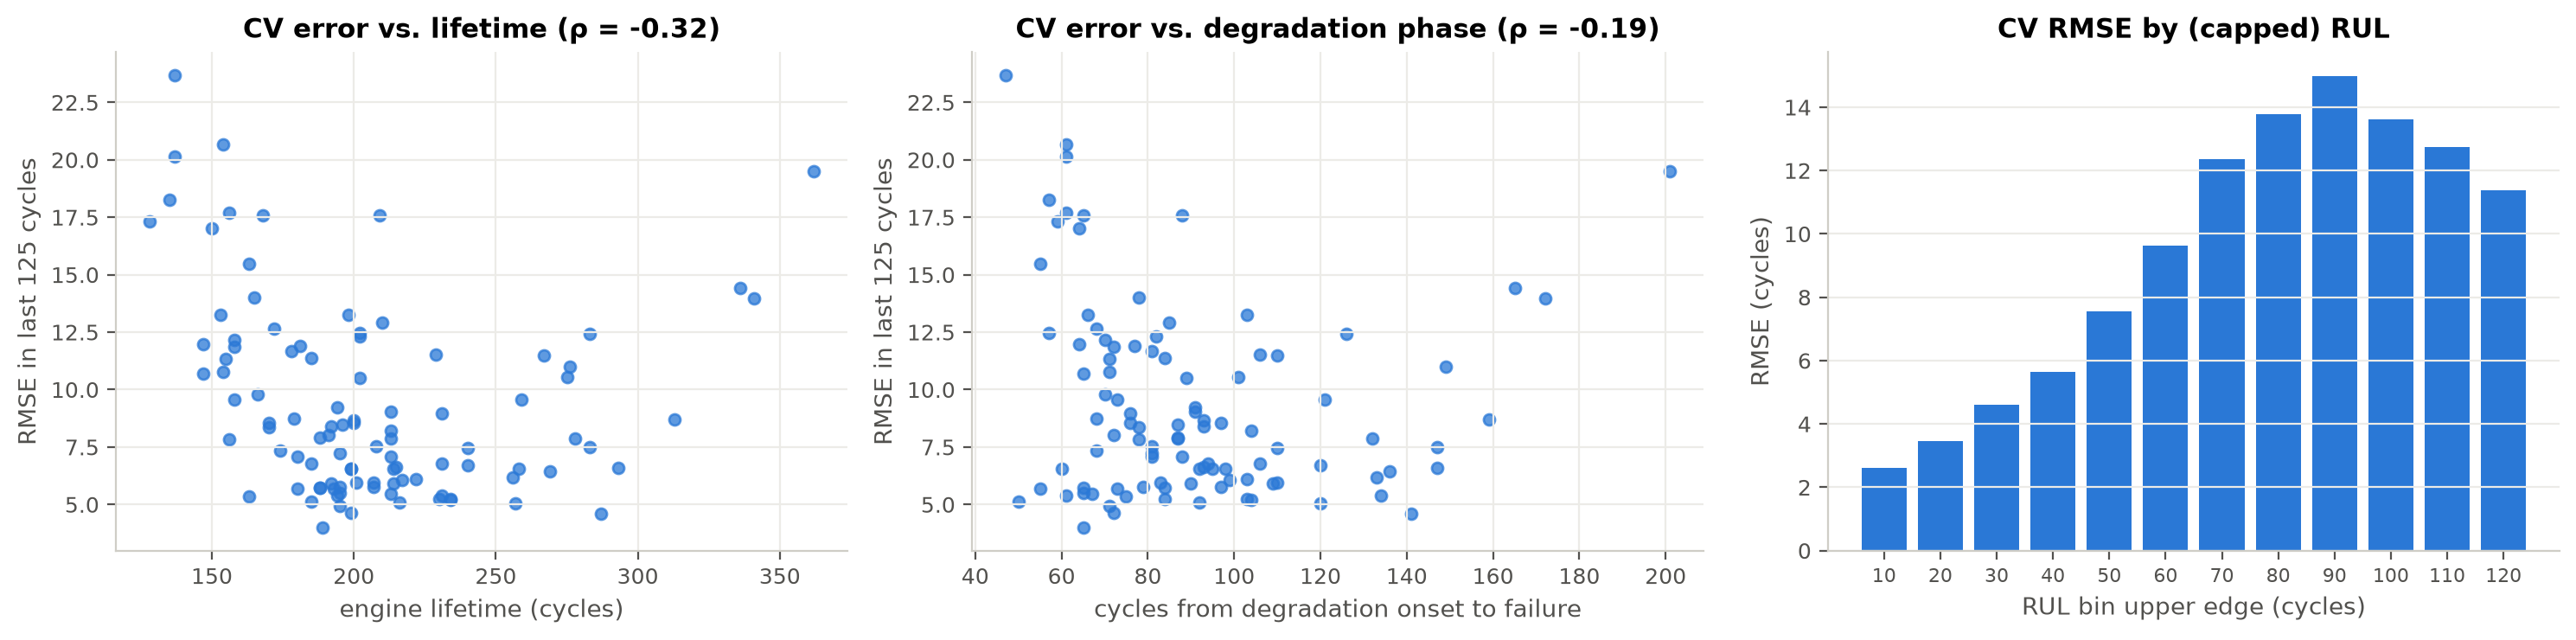
\includegraphics[width=0.92\textwidth]{05_gap_analysis.png}
  \caption{Error analysis on out-of-fold CV predictions (XGBoost): per-engine error vs.\ lifetime and vs.\ length of the degradation phase, and RMSE by RUL bin.}
  \label{fig:gap}
\end{figure*}

\textbf{Limitations.} FD001 is simulated, has one operating condition and one fault mode, and its test set has only 100 engines, so the confidence intervals are wide (about $\pm1.7$ cycles). Our tuned cross-validation scores are slightly optimistic because the same folds were used for selection. The test set, used only once, gives the unbiased estimate.

%=====================================================================
\section{Conclusion}
%=====================================================================
On C-MAPSS FD001, a leakage-free pipeline of degradation features with gradient boosting predicts RUL with a test RMSE of 10.75 cycles, and only 5.7 cycles in the last 50 cycles before failure. The decisive ingredients are a piecewise-linear target and features that describe each engine relative to its own history (baseline deviation, trend slopes and a health index). Hyperparameter tuning matters far less. The remaining errors concentrate on fast degraders, the onset of degradation and short histories, all of which motivate sequence models in Phase~2, which can also extend the regime-aware pipeline to FD002--FD004.

%=====================================================================
\section*{Team Contributions}
%=====================================================================
{\small
\begin{tabular}{p{0.25\columnwidth}p{0.6\columnwidth}}
\toprule
Member & Responsibility \\
\midrule
Kushal Tyagi & Project lead; modelling, cross-validation and tuning; test evaluation and error analysis (notebooks 04--05, \texttt{src/models.py}, \texttt{src/evaluation.py}); documentation \\
Nishant Sharma & Exploratory analysis and feature engineering (notebooks 02--03, \texttt{src/features.py}) \\
Anant Lalwani & Literature review and report; data loading and quality checks (notebook 01) \\
Dev Tyagi & Data set sourcing and documentation (\texttt{data/}, download script) \\
Vansh Khod & Data cleaning and validation (data-integrity tests) \\
\bottomrule
\end{tabular}}

\vspace{4pt}
\noindent Code and notebooks: \url{https://github.com/WhiteHacker000/Remaining-Useful-Life-Prediction-for-Industrial-Engines}

\bibliographystyle{IEEEtran}
\bibliography{references}

\end{document}
